\documentclass[10pt,sans,english,compress,table,xcolor=dvipsnames]{beamer}
\author[Lily ]{ Dr Lily Asquith (Lily, she/her)}

\usetheme{Szeged}
%\defbeamertemplateparent{enumerate items}{enumerate item,enumerate subitem,enumerate subsubitem,enumerate mini template}
\definecolor{titcol}{RGB}{16,78,100} 
\setbeamercolor{frametitle}{fg=titcol,bg=White}
\useoutertheme{miniframes} 
\useinnertheme{rectangles}

\usepackage{pifont}
\newcommand{\tick}{\textcolor{grn}{\ding{52} } }
\newcommand{\nope}{\textcolor{red}{\ding{54} } }


\usepackage{soul}
\usepackage{cancel}

\usepackage[most]{tcolorbox}
\definecolor{LilyBlack}{rgb}{0.05,0.1,0.3} % UBC Blue (primary)
\usecolortheme[named=LilyBlack]{structure}

\usepackage{booktabs}
\usepackage{tabularx}
%\usepackage{tikz}
%\def\checkmark{\tikz\fill[scale=0.4](0,.35) -- (.25,0) -- (1,.7) -- (.25,.15) -- cycle;}

\usepackage{physics}

\usepackage{xparse}

\setbeamertemplate{footline}{%
  \leavevmode%
  \hbox{\begin{beamercolorbox}[wd=.5\paperwidth,ht=2.5ex,dp=1.125ex,leftskip=.3cm plus1fill,rightskip=.3cm]{author in head/foot}%
    \usebeamerfont{author in head/foot}\insertshortauthor
  \end{beamercolorbox}%
  \begin{beamercolorbox}[wd=.5\paperwidth,ht=2.5ex,dp=1.125ex,leftskip=.3cm,rightskip=.3cm plus1fil]{title in head/foot}%
    \usebeamerfont{title in head/foot}\insertshorttitle\hfill\insertframenumber\,/\,\inserttotalframenumber
  \end{beamercolorbox}}%
  \vskip0pt%
}

\DeclareMathSizes{10}{10}{6}{4} % this one
%\DeclareMathSizes{10.95}{10}{6}{4}   % For size 10 text

\newcommand*\ColorBox[3][black]{%
  \makebox[2em][c]{%
    \setlength\fboxsep{-.5\fboxrule}%
    \raisebox{\dimexpr-#3em+.5ex}{%
      \fcolorbox{#1}{#2}{%
        \rule{0pt}{\dimexpr#3em*2}%
        \rule{\dimexpr#3em*2}{0pt}%
      }%
    }%
  }%
}

\usepackage{hyperref}
\hypersetup{
    colorlinks=true,
    linkcolor=blue,
    filecolor=magenta,      
    urlcolor=blue,
    pdftitle={Overleaf Example},
    pdfpagemode=FullScreen,
    }

\urlstyle{same}

% this part excludes specified frames from counters in navigation bar
\makeatletter
\let\beamer@writeslidentry@miniframeson=\beamer@writeslidentry
\def\beamer@writeslidentry@miniframesoff{%
  \expandafter\beamer@ifempty\expandafter{\beamer@framestartpage}{}% does not happen normally
  {%else
    % removed \addtocontents commands
    \clearpage\beamer@notesactions%
  }
}
\newcommand*{\miniframeson}{\let\beamer@writeslidentry=\beamer@writeslidentry@miniframeson}
\newcommand*{\miniframesoff}{\let\beamer@writeslidentry=\beamer@writeslidentry@miniframesoff}
\makeatother


\makeatletter
\newcommand\notsotiny{\@setfontsize\notsotiny{6.5}{7.5}}
\makeatother




\usepackage{multicol}
\usepackage{sansmath}
\usepackage{minted}
\definecolor{LightGray}{gray}{0.95}
\definecolor{lgreen}{rgb}{0.59, 0.87, 0.82}
\definecolor{lpink}{rgb}{0.98, 0.85, 0.87}

\usepackage{array}
\newcolumntype{L}{>{$}l<{$}}
\newcolumntype{C}{>{$}c<{$}}

\title[Funcs]{Probability Functions}
\date{}
\titlegraphic{
%\center

\includegraphics[scale=0.15]{sussex-logo}
}

%\newcommand{\rvX}[1]{ X_{ {#1} } 
%\newcommand{\rvY}[1]{ Y_{ {#1} }



\begin{document}

\newcommand\info{\mathcal{J}_{\theta}}
\newcommand\loglike{\ln{ \mathcal{L}_{\theta}} }
\newcommand\like{\mathcal{L}_{\theta} }

\newcommand\thetahat{\hat{ \theta }  }

\definecolor{grn}{RGB}{0,128,0} 
\newcommand{\gbl}[1]{\textcolor{grn}{#1}}

\definecolor{wh}{rgb}{0.95, 0.95, 0.96}
\newcommand{\wht}[1]{\textcolor{wh}{#1}}

%\newcommand{\inprob}{\overset{p}{\to}}

\newcommand{\boo}[1]{\textbf{\textcolor{red}{#1}}}

\newcommand{\covmat}{\mathbf{\textcolor{magenta}{\Sigma}} }


\definecolor{purr}{RGB}{128,0,128} 
\newcommand{\purp}[1]{\textcolor{purr}{#1}}

\newcommand{\magt}[1]{\textbf{\textcolor{magenta}{#1}}}
 \newcommand{\magtn}[1]{\textcolor{magenta}{#1}}
 
%\definecolor{bbl}{RGB}{128,0,128} 
\newcommand{\bbl}[1]{\textcolor{blue}{#1}}

\newcommand{\rbl}[1]{\textcolor{red}{#1}}

\definecolor{dblu}{RGB}{37,150,190} 
\newcommand{\blu}[1]{\textcolor{dblu}{#1} }

\definecolor{dor}{RGB}{255,40,0} 
\newcommand{\dor}[1]{\textcolor{dor}{#1} }

\definecolor{darkgreen}{RGB}{46,139,87} 
\newcommand{\dgreen}[1]{\textbf{\textcolor{darkgreen}{#1}} }
%\newcommand{\gbl}[1]{\textcolor{darkgreen}{#1}}

\definecolor{lgray}{RGB}{222,222,222} 

\definecolor{lyellow}{RGB}{255,255,224} 

\newcommand{\E}[1]{\mathbf{E}_{#1}}
%
\newcommand{\rvX}[1]{X_{(#1)} } 

\newcommand{\rvY}[1]{Y_{(#1)} }

\newcommand{\rvx}[1]{x_{(#1)} } 

\newcommand{\rvy}[1]{y_{(#1)} }



\newcommand{\red}[1]{\textcolor{red}{#1} }

\newcommand{\bluedots}{\blu{\ldots} }

\newcommand{\dordots}{\dor{\ldots} }


\newcommand{\where}{\dgreen{\;where\;} }


\newcommand{\pand}{\dgreen{\;and\;} }
\newcommand{\por}{\dgreen{\;or\;} }

\newcommand{\sumN}{ \sum\limits_{\blu{i}}^{\blu{N}} }

\newcommand{\sumZ}{ \sum\limits_{\dor{j}}^{\dor{Z}} }

\newcommand{\Expec}[1]{ \mathbb{E}[#1] }


\newcommand{\Xfj}[1]{ X_{ \dor{#1} } }

\newcommand{\xfi}[1]{ x_{ \blu{#1} } }

\newcommand{\Xij}[2]{ X_{\mage{#1},\blu{#2} }}

\newcommand{\sumxi}{ \sumN \xfi{i} }

\newcommand{\sumXj}{ \sumZ \Xfj{j} }

\newcommand{\sumZa}[1]{ \sumZ {#1}_{ \dor{j} } }

\newcommand{\sumZab}[2]{ \sumZ {#1}_{ \dor{j} }\, {#2}_{ \dor{j} } }

\newcommand{\sumNab}[2]{ \sumN {#1}_{ \blu{i} }\, {#2}_{ \blu{i} } }

\newcommand{\vecxi }{ [ \xfi{1} \xfi{2}, \bluedots, \xfi{N} ] }

\newcommand{\vecXj }{ [ \Xfj{1} \Xfj{2}, \bluedots, \Xfj{Z} ] }

\newcommand{\vecXij }{ [ \Xij{1}{1} \Xij{1}{2}, \bluedots, \Xij{1}{N_1} ],\, [ \Xij{2}{1} \Xij{2}{2}, \bluedots, \Xij{2}{N_2} ],\, \dordots,\,[ \Xij{Z}{1} \Xij{Z}{2}, \bluedots, \Xij{Z}{N_Z} ] }

% definitions

\newcommand{\overNblack}{ \dfrac{1}{N} }
\newcommand{\overN}{ \dfrac{1}{ \blu{N} } }

\newcommand{\defmean }{ \overline{x} = \overN \sumN \xfi{i} }

\newcommand{\meanx }{ \overline{x} }
\newcommand{\meansqx }{ \overline{x^2} }
\newcommand{\sqmeanx }{ \overline{x}^2 }
\newcommand{\devsq}{ (\xfi{i} - \meanx)^2 }

%\newcommand{\var }[1]{ \mathcal{V}_{#1} }
\newcommand{\defvar }{ \var{x} = \overN \sumN \devsq }
\newcommand{\defvarshort }{ \var{x} = \meansqx - \sqmeanx }

\newcommand{\defstd }{ s_x = \sqrt{ \var{x} }  }

\newcommand{\defwmean }{ \overline{X} = \dfrac{ \sumZab{w}{X} }{ \sumZa{w} } }  

\newcommand{\defw }{ w_{\dor{j}} = \dfrac{1}{ \var{\Xfj{j} } } }



\begin{frame}
\titlepage
\end{frame} 

%\section*{Preamble}
\begin{frame}{Assignment Notes} 
Hopefully you have all decided on either the \boo{Visualising Bayes} or \boo{Explaining Monty Hall} options for the first assignment.\\[1ex]

I finally found time to do the Visualizing Bayes option, and found that I could make the plot more informative by choosing different values from those specified on the assignment. It is fine if you go `off piste' a  little bit with those instructions, if you want to. \\[1ex]

For the Monty Hall one-pager, I have uploaded an example latex template and it is also fine to use a google doc if latex is not useful for your future.\\[1ex]
\end{frame}


\begin{frame}{The Monty Hall Problem \boo{pollev.com/ilovephysics}} 

Suppose you're on a game show, and you're given the choice of three doors. Behind one door is a car, behind the others, goats. You pick a door, say $\#1$, and the host, who knows what's behind the doors, opens another door, say $\#3$, which has a goat. He says to you, `Do you want to pick door $\#2$?' Is it to your advantage to switch your choice of doors?\\[1ex]
\vspace{4cm}


\end{frame}



% python
\begin{frame}[fragile]{Following with Python}


Download the notebook from the canvas page for this week's material: \dgreen{Funcs.py} \\[1ex]

\begin{minted}[bgcolor=LightGray]{python}
marimo edit Funcs.py
\end{minted}

\end{frame} 

% contents
\begin{frame}{Probability Functions}
\large
\begin{itemize}
\item Probability Mass \& Density Functions\\[1ex]
\item Parameters\\[1ex]
\item Cumulative Distributions\\[1ex]
\item Joint PDF\\[1ex]
\item Likelihood\\[1ex]
\item Transforms, Jacobian\\[1ex]
\end{itemize}

\end{frame} 

%Distributions
\section*{PMFs/PDFs}

% slide
\begin{frame}{Probability Distributions}

A Probability Distribution Function is a function of one or more RVs and one or more parameters, and represents the probability of all the ranges of values the RV can take.\\[1ex]

If the RV is:\\[1ex]
\boo{Discrete}: the distribution is a \boo{Probability Mass Function}: a set of points.\\[1ex]
\boo{Continuous}: the distribution is a \boo{Probability Density Function}: a smooth curve.\\[1ex]

\blu{Note that Probability Distribution Functions are very often referred to as PDFs. Overloaded term also used for Probability Density Function.} \\[1ex]
 
%We will see that there are a large number of these PDFs and PMFs, and will barely mention where they "came from". 

%PDFs and PMFs  arose over time as a result of human beings observing the world and noticing that natural phenomen\boo{*} seemed to occur according to different underlying sets of rules. \\[1ex]

% \boo{*}In reality I expect that the natural phenomena were more likely related to gambling games than to eg astronomical observations. 
\end{frame} 


%DATA
\begin{frame}{Discrete versus Continuous: Examples}

\boo{Discrete RVs} \hspace{5cm} \boo{Continuous RVs}\\[1ex]

\vspace{4cm}

\blu{Note that measured data is always discrete, no matter the nature of the underlying RV.}\\[1ex]
\end{frame}

% PMF
\begin{frame}{Probability Mass Functions}

A Probability Mass Function (\boo{PMF}) is $p_X$ where $X=X_{(1)}$ is a single discrete RV.\\[1ex]

The \boo{Support} S of a PMF (also PDF) is the set of all values with a non-zero probability of occurring.\\[1ex]

A PMF must satisfy three conditions:\\
\blu{
\begin{itemize}
\item[1]  $p_X(x) > 0\;\;\; \forall\;\; x \in S$\\[2ex]
\item[2]  $\sum\limits_{x\in S} p_X(x) =1$\\[2ex]
\item[3]  $ P(x \in A) = \sum\limits_{x\in A} p_X(x) $\\[2ex]
\end{itemize}
}
\end{frame} 


\begin{frame}{Discrete PMF Example: max score from two dice}
\small

Sample space is $S=\{ (i,j) | i,j=1,2,3,4,5,6 \}$: there are $i\cdot j$=36 possible outcomes with equal probability.\\[1ex]

The total probability is 1, and is the sum of the individual probabilities, so $p_{ij} = \dfrac{1}{36}$.\\[1ex]

Some outcomes will appear more than once.\\[1ex]
\begin{multicols}{2}

\footnotesize
\begin{tabular}{L|*{6}{L}} 
\mathsf{i,j} & 1 & 2 & 3 & 4 & 5 & 6\\
\hline
1 & \cellcolor{LightGray}1 & \cellcolor{lgreen}2 & \cellcolor{lpink}3 & 4 & 5 & 6\\
2 &  \cellcolor{lgreen}2& \cellcolor{lgreen}2 &  \cellcolor{lpink}3& 4 &5  &6 \\
3 &  \cellcolor{lpink}3&  \cellcolor{lpink}3&  \cellcolor{lpink}3 &  4 &5  &6 \\
4 &  4&  4&  4  & 4 &5  &6 \\
5 &  5&  5&  5 &   5&  5 & 6 \\
6 &  6&  6&  6 & 6  & 6 & 6\\
\end{tabular}

\begin{tabular}{C| *{7}{C}} 
\mathsf{X} & \cellcolor{LightGray}1 &  \cellcolor{lgreen}2 & \cellcolor{lpink}3 & 4 & 5 & 6\\
\mathsf{p_X} &\cellcolor{LightGray} \frac{1}{36} &   \cellcolor{lgreen}\frac{3}{36} &  \cellcolor{lpink}\frac{5}{36} &  \frac{7}{36}  &  \frac{9}{36}  &  \frac{11}{36} \\
\end{tabular}

\end{multicols}
\end{frame}


\begin{frame}{Discrete PMF Example: max score from two dice}
\small
\centering
\begin{tabular}{C| *{7}{C}} 
\mathsf{X} & \cellcolor{LightGray}1 &  \cellcolor{lgreen}2 & \cellcolor{lpink}3 & 4 & 5 & 6\\
\mathsf{p_X} &\cellcolor{LightGray} \frac{1}{36} &   \cellcolor{lgreen}\frac{3}{36} &  \cellcolor{lpink}\frac{5}{36} &  \frac{7}{36}  &  \frac{9}{36}  &  \frac{11}{36} \\
\end{tabular}

%\centering
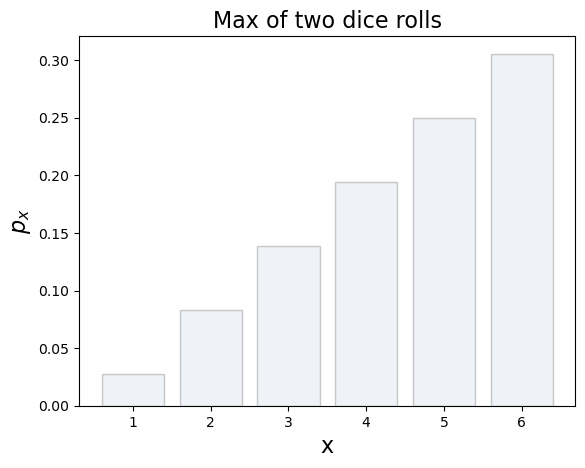
\includegraphics[scale=0.4]{PMF-MaxDice.png}

\end{frame}

% PDF
\begin{frame}{Probability Density Functions}

A Probability Density Function (\boo{PDF}) is $f_X$ where $X=X_{(1)}$ is a single continuous RV.\\[1ex]

%The \boo{Support} S of a PDF is the set of all values with a non-zero probability of occurring\\[1ex]

A PDF must satisfy the same conditions as a PMF, but we write the second and third in terms of integrals:\\[1ex]
\begin{itemize}
\item[1]  $f_X(x) > 0\;\;\; \forall\;\; x \in S$\\[2ex]
\item[2]  $\int\limits_{S} f_X(x)\,dx =1$\\[2ex]
\item[3]  $ P(x \in A) = \int\limits_{A} f_X(x)\, dx $\\[2ex]
\end{itemize}
\end{frame} 

% Area
\begin{frame}{Probability: Area under distribution}

\textbf{Note that for a continuous RV $X$, the value of the PDF at some value of $X=x$ is not the probability of that value.} The absolute $y-axis$ value of a PDF has no meaning.\\[1ex]

\blu{Recall that $\int\limits_{-\infty}^{\infty} f_X dx = 1$, so $f_X$ at any of the infinite possible values must be infinitesimally small: zero.}\\[1ex]

Trying to extract the probability of any exact value from a continuous PDF will return zero. \\[1ex]

\boo{For continuous RVs, we can only talk about the probability of a value in a given range.}

%To get the probability of some value from a PDF we must supply a range around that value (and use the \boo{CDF}, up in a sec.) \\[1ex]
\end{frame} 

% Total is one
\begin{frame}{The Total Probability $\int\limits_{S} f_X(x)\,dx =1$}
Spot the difference:\\[1ex]
\center
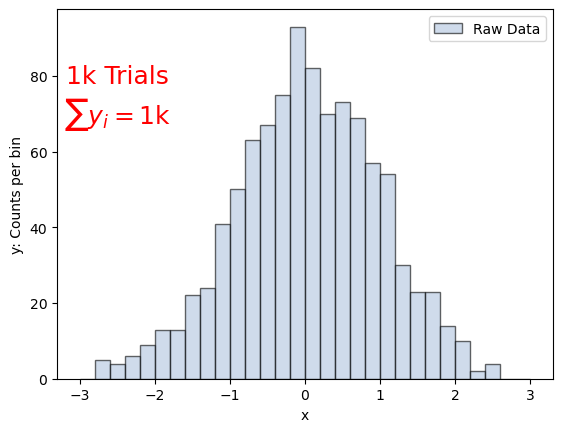
\includegraphics[scale=0.35]{PLOTDAT3-NormToPDF-Raw.png}
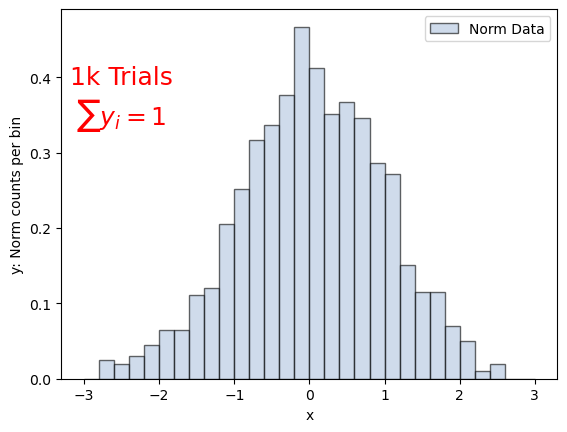
\includegraphics[scale=0.35]{PLOTDAT3-NormToPDF-Norm.png}

\end{frame} 

% Total is one
\begin{frame}{The Total Probability $\int\limits_{S} f_X(x)\,dx =1$}

\center
This is a regular distribution \hfill \boo{This is a Probability Distribution}\\[1ex]
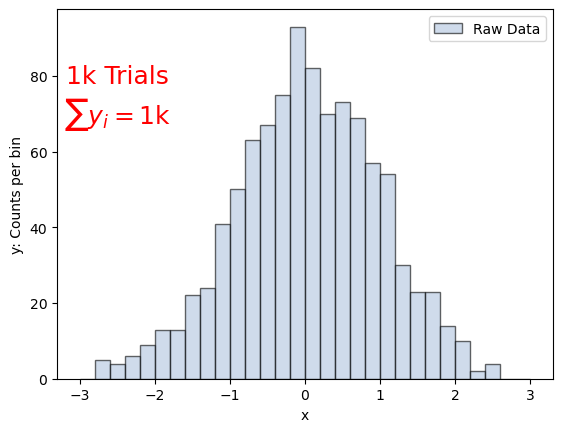
\includegraphics[scale=0.35]{PLOTDAT3-NormToPDF-Raw.png}
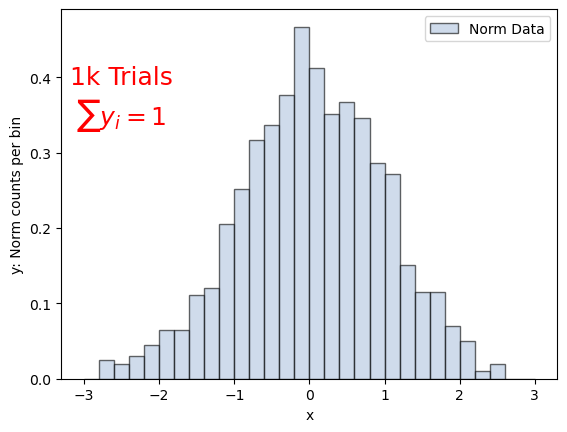
\includegraphics[scale=0.35]{PLOTDAT3-NormToPDF-Norm.png}

A PDF/PMF must be Normalised to unity, otherwise it does not satisfy the second axiom.
\end{frame} 

% Normalisation
\begin{frame}{Reminder: Normalisation}
Any function of a continuous RV can be turned into a PDF. For example: \\[1ex]
\boo{ $f(X;\theta) = x^3$ is a function}\\[1ex]
\begin{itemize}
\item[1] Write $f(X;\theta) = A x^3$\\[1ex]
\item[2] Specify the `range', for example $X:[0,1]$\\[1ex]
\item[3] Set integral to one: $\int\limits_0^1   A x^3 dx =1$\\[1ex]
\item[4] Solve for A:  $A \dfrac{1}{4} =1 \therefore A= 4 $\\[2ex]
\end{itemize} 
\boo{$f_X = 4x^3$ for $0\leq x \leq 1$ is a valid PDF}\\[1ex]

\end{frame} 


\section*{Parameters}

%param
\begin{frame}[fragile]{Parameters}
The \boo{Parameters} $\theta$ of a PDF or PMF are classified by how they modify the behaviour of the function wrt the RV(s)\\

\blu{Consider a curve of some sort (a distribution function). If you move it to the left or right, it is still the same curve: has it shifted, or has the x-axis?}\\

How about if you squish it or stretch it a bit?\\

\center
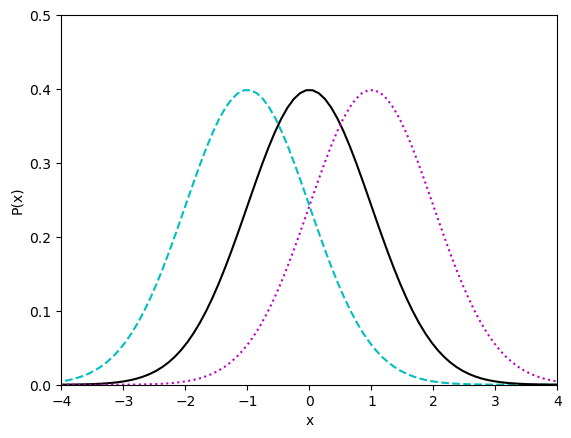
\includegraphics[scale=0.33]{Params-Location.png} 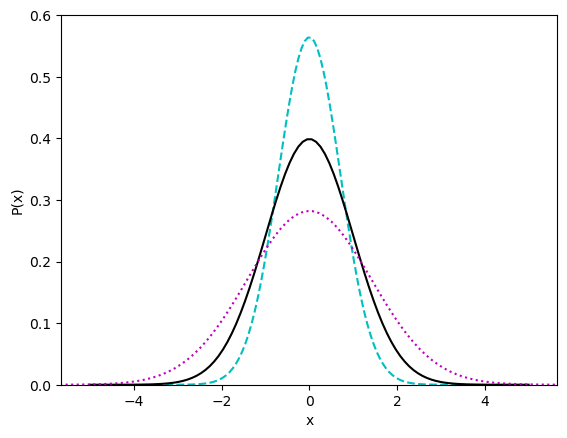
\includegraphics[scale=0.33]{Params-Scale.png}

\end{frame} 

%param
\begin{frame}[fragile]{Location Parameter}
The \boo{Location Parameter} of a PDF or PMF sets its position on the $x$-axis\textcolor{magenta}{*}.\\[1ex]

\center
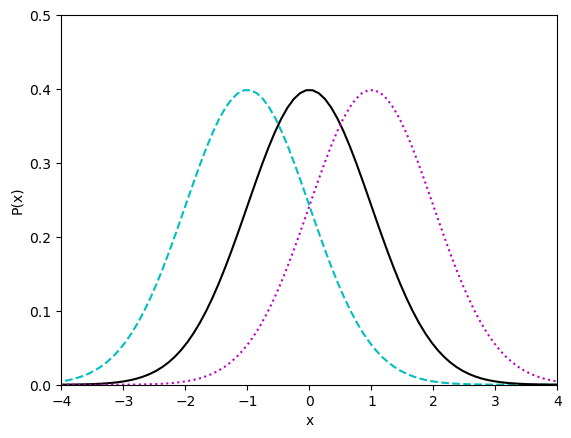
\includegraphics[scale=0.35]{Params-Location.png}

\blu{For the Gaussian PDF in this example, the location parameter is $\mu$, the True Mean.}\\[1ex]
\end{frame} 


%param
\begin{frame}[fragile]{Scale Parameter}
The \boo{Scale Parameter} of a PDF or PMF sets its spread on the $x$-axis\textcolor{magenta}{*}.\\[1ex]


\center
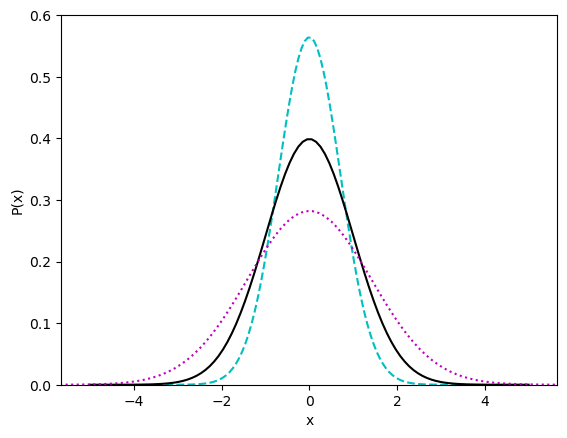
\includegraphics[scale=0.35]{Params-Scale.png}

\blu{For the Gaussian PDF in this example, the scale parameter is $\sigma$, the Standard Deviation.}\\[1ex]
\end{frame} 


%\begin{frame}[fragile]{Python}
%Example python code with loc and scale parameters:\\[1ex]
%
%\begin{minted}[bgcolor=LightGray]{python}
%from scipy.stats import norm
%import matplotlib.pyplot as plt
%mu = 0
%lines = ['c--', 'k-', 'm:']
%sigmas = [0.5,1,2]
%x = np.linspace(-5,5, 100)
%for l,sigma in zip(lines,sigmas):             
%        y = norm.pdf(x, loc=mu, scale=sigma)
%        plt.plot(x, y, l)
%plt.show()
%\end{minted}
%\end{frame} 



\begin{frame}[fragile]{\textcolor{magenta}{*}Simplification Warning}

Consider a PDF  $f_X(X;\theta) = \theta_s(x-\theta_L)$.\\[1ex]
The two parameters are $\theta=\{\theta_s,\theta_L\}$. The Scale Parameter is $\theta_s$ and the location parameter is $\theta_L$\\[1ex]
The inverse of a \boo{Scale Parameter} is called a \boo{Rate Parameter}\\[1ex]

\textbf{Note that the shifting and squishing/stretching analogy above is a pedagogic simplification.}\\[1ex]
 \blu{Distribution functions often have forms like $f_X \propto \lambda^X$  (cf Poisson), where the parameter $\lambda$ is a Rate Parameter (which we defined as squish/stretch) that also shifts the distribution peak left and right (which in our oversimplification we claimed was the job of the Location Parameter).}

\end{frame}

\begin{frame}[fragile]{Normalisation versus Scale}

We saw that $f_X = 4x^3$ is a valid PDF because it has integral 1.\\[1ex]

My simplified explanation of the scale parameter might lead you to believe that using it could ruin the validity of the PDF.\\[1ex]

Scale and Location parameters cannot `break' the normalisation of a PDF.\\[1ex]

The normalisation is not optional. It is fixed. If we change the scale/location, the range of validity (the domain) must also change.\\[1ex]

\end{frame}



\begin{frame}[fragile]{Shape Parameter, Examples}
The \boo{Shape Parameter} alters the curve more profoundly, causing the peak to move while also affecting the symmetry of the distribution. \\[1ex]

\small
\textbf{More on this}: The Gaussian does not have a shape parameter, but there are PDFs that do (Beta, T, ..): please enjoy this fantastic interactive page: \href{https://www.acsu.buffalo.edu/~adamcunn/probability/normal.html}{Probability Playground} . It allows you to change the parameters of pretty much any distribution you can think of. \\[1ex]

\textbf{Scipy}: The scale and loc parameters are used in the \href{https://docs.scipy.org/doc/scipy/reference/stats.html}{scipy stats library}, which has an extensive range of probability distributions. The scipy stats distribution functions can also take parameters as arguments which are not strictly classified as scale or loc. An example of a distribution like this is the Binomial, which we will cover soon. Its parameters do shift and squish/stretch the distribution, but they don't \textit{only} shift and stretch/squish the distribution.

\end{frame}



\section*{CDFs}

% discrete CDF

\begin{frame}{Cumulative Distribution Function}
A \boo{CDF} (Cumulative Distribution Function) $F_X$  allows us to calculate the probability of $X$ being measured as \textbf{any value up to and including a given value}.\\[2ex]
%I use the notation $F_X$ for a CDF:\\[1ex]
$F_X(x) = P(X\leq x)  = \sum\limits_{x_i\leq x} p_X(x_i)$ : \boo{CDF}  for Discrete $X$\\[1ex]

Example: $X$ is the maximum value from rolling two dice\\[1ex]

\footnotesize

\begin{tabular}{C| *{7}{C}} 
\mathsf{X} & \cellcolor{LightGray}1 &  \cellcolor{lgreen}2 & \cellcolor{lpink}3 & 4 & 5 & 6\\[1ex]
\mathsf{p_X} &\cellcolor{LightGray} \frac{1}{36} &   \cellcolor{lgreen}\frac{3}{36} &  \cellcolor{lpink}\frac{5}{36} &  \frac{7}{36}  &  \frac{9}{36}  &  \frac{11}{36} \\[1ex]
\mathsf{F_X} &\cellcolor{LightGray} \frac{1}{36} &   \cellcolor{lgreen}\frac{4}{36} &  \cellcolor{lpink}\frac{9}{36} &  \frac{16}{36}  &  \frac{25}{36}  &  \frac{36}{36} \\
\end{tabular}
\vspace{0.5cm}

\normalsize
$F_X(4) = P(X\leq 4)  =  \dfrac{16}{36}$\\[1ex] 

\end{frame}






\begin{frame}{CDF: Continuous RV}
A \boo{CDF} (Cumulative Distribution Function) $F_X$  allows us to calculate the probability of $X$ being measured as \textbf{any value up to and including a given value}.\\[2ex]

$F_X(x) = P(X\leq x)  = \int\limits_{-\infty}^{x} f_X(x)\,dx$ : \boo{CDF}  for Continuous $X$\\[1ex]
 
%The result of the integral gives us the probability of any measured value up to and including $x$.\\[1ex]

Recall: \boo{For continuous RVs, we can only talk about the probability of a
value in a given range.}


%To calculate the probability of a value occuring, eg $x=5$,  we evaluate the CDF \textbf{just above and below} ($\delta$:tiny amount) this value, and subtract:\\[1ex]
%$P(X=x) \rightarrow  P(X< (x+\delta) ) - P(X< (x-\delta) )$\\[1ex]
 


\end{frame}



\begin{frame}[fragile]{PDF and CDF}

\textcolor{blue}{$f_X$  : PDF gives us a shape.}\\[1ex]
\textcolor{red}{$F_X = \int\limits_{-\infty}^{x} f_X(x)\,dx= P(X\leq x)  $}: CDF gives us a Probability\\[1ex]

\center
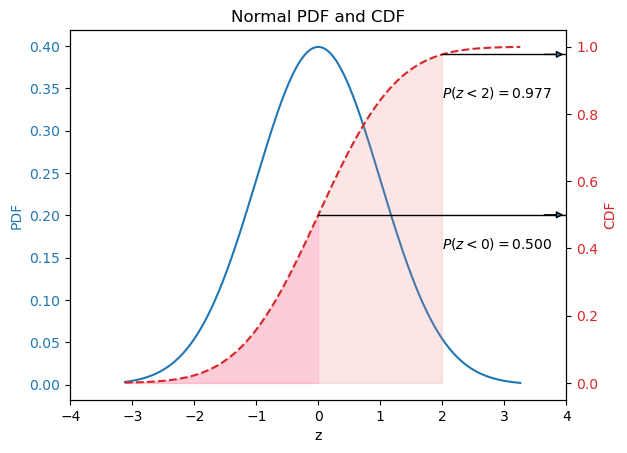
\includegraphics[scale=0.38]{PLOTDAT3-NormalPDFandCDF.png}


\end{frame}

\begin{frame}[fragile]{Properly defining the PDF}
The PDF we made earlier is $f_X = 4x^3$ for $0\leq x \leq 1$. \\[1ex]
To properly define this PDF, we need to also specify what it does outside the range $0\leq x \leq 1$:\\[1ex]

\begin{equation}\nonumber
f_X(x) = 
\begin{cases}
     0\; & x < 0\\[1ex] 
  4x^3\; & 0\leq x \leq 1 \\[2ex]
  0\; & x>1 \\[2ex]
\end{cases}
\end{equation}


\end{frame}


\begin{frame}[fragile]{Properly defining the continuous CDF}
The CDF is $F_X(x) = \int_{-\infty}^{x} f_X(x) \,dx$ \\[1ex]

For this $f_X = 4x^3$ we have three regions. \\[1ex]

$F_X(x) = \int_{x<0} f_X(x) \,dx + \int_{0}^{1} f_X(x) \,dx + \int_{x>1} f_X(x) \,dx$

\begin{equation}\nonumber
F_X(x) = 
\begin{cases}
     0\; & x < 0\\[1ex] 
  x^4\; & 0\leq x \leq 1 \\[2ex]
  0\; & x>1 \\[2ex]
\end{cases}
\end{equation}
\end{frame}


\begin{frame}[fragile]{Probability for a CRV}
\begin{equation}\nonumber
F_X(x) = 
\begin{cases}
     0\; & x < 0\\[1ex] 
  x^4\; & 0\leq x \leq 1 \\[2ex]
  0\; & x>1 \\[2ex]
\end{cases}
\end{equation}

The Probability of $X\leq0.1$:\\[1ex]
$F_X(0.1) = \textcolor{red}{\int\limits_{-\infty}^{0} 4x^3 \,dx} + \int\limits_{0}^{0.1} 4x^3 \,dx = \textcolor{red}{0}+ x^4\bigg|^{0.1}_{0} = 0.1^4 -0 = 0.0001$\\[2ex]


\end{frame}

\begin{frame}[fragile]{Probability for a CRV}
\begin{equation}\nonumber
F_X(x) = 
\begin{cases}
     0\; & x < 0\\[1ex] 
  x^4\; & 0\leq x \leq 1 \\[2ex]
  0\; & x>1 \\[2ex]
\end{cases}
\end{equation}

The Probability of $0.45< X\leq 0.55$:\\[1ex]
$F_X(0.45) =  \int\limits_{0}^{0.45} 4x^3 \,dx =  x^4\bigg|^{0.45}_{0} = 0.45^4 -0 $\\[2ex]
$F_X(0.55) =  \int\limits_{0}^{0.55} 4x^3 \,dx =  x^4\bigg|^{0.55}_{0} = 0.55^4 -0 $\\[2ex]

$F_X(0.55)- F_X(0.45) =  0.55^4 - 0.45^4 = 0.0505$\\[1ex]


\end{frame}

\begin{frame}[fragile]{Probability for a CRV}
\begin{equation}\nonumber
F_X(x) = 
\begin{cases}
     0\; & x < 0\\[1ex] 
  x^4\; & 0\leq x \leq 1 \\[2ex]
  0\; & x>1 \\[2ex]
\end{cases}
\end{equation}

The Probability of $X>0.95$:\\[1ex]
$F_X(0.95) =  \int\limits_{0.95}^{1} 4x^3 \,dx =  x^4\bigg|^{1}_{0.95} = 1 - 0.95^4 = 0.1855 $\\[2ex]


\end{frame}







\section*{Joint/Marginal PDF}

\begin{frame}{Joint Probability}
The \boo{Joint CDF} for two RVs ${Y,Z}$ allows us to calculate the joint probability of the two RV measurements.\\[1ex]
 
 $P(\{\blu{Y =y}\}\,\cap\,\{\blu{Z=z}\}) = F_{YZ}(y,z;\theta)$\\[1ex]
 
A Joint PDF must satisfy:\\
\blu{
\begin{itemize}
\item[1]  Normalisation: $0 \leq f_{YZ} \leq 1$ \\[2ex]
\item[2]  Total probability must be 1: $\int\limits_{-\infty}^{\infty} \int\limits_{-\infty}^{\infty} f_{YZ}\, dy\, dz =1 $\\[2ex]
\end{itemize}
}
\blu{Note that $Y=y$ is shorthand for $(y-\delta) \leq Y \leq (y+\delta)$}\\[1ex]
\end{frame}



\begin{frame}{Joint Probability for two Independent RVs}

$P(\{Y =y\}\,\cap\,\{Z=z\}) = F_{YZ}(y,z;\theta)$\\[1ex]

Recall the  Conditional Probability: $P(A\, \cap\, B) = P(A\, |\, B) P(B) $\\[1ex]

If the RVs are Independent, this is $P(A\, \cap\, B) = P(A ) P(B) $\\[1ex]

In that case, we can write the \boo{Joint PDF for Independent RVs}:\\[1ex] 

 $ f_{YZ}(y,z;\theta) = f_{y}(y;\theta) \, f_Z (z;\theta) $\\[1ex]
 
 \blu{The independence allows us to factorise the joint PDF into a product of the PDFs for the individual RVs.}\\[1ex]

\end{frame}


\begin{frame}{Independent RVs}

Two random variables $Y$ and $Z$ are independent if knowing the value of one of them does not change the probabilities for the other one.\\[1ex]

Are these pairs \boo{Independent}, \boo{Dependent}, or \boo{Need to look into that}\\[1ex]

\begin{itemize}
\item $Y$: coin toss, $Z$: another coin toss\\[1ex]
\item $Y$: speed of a car, $Z$: kinetic energy of a car\\[1ex]
\item $Y$: my assigned sex, $Z$: my IQ\\
\end{itemize}


\vspace{2cm}

\end{frame}





\begin{frame}{Joint PDF: Example}

Suppose $Y$ and $Z$ have values in [0,1] with $f_{YZ}(y,z) = 4yz$.\\[1ex]

Check $f_{YZ}$ is a valid:\\[1ex]
$
\int \limits_{0}^{1}  \int \limits_{0}^{1}\,4yz\, dy\, dz = 
\int \limits_{0}^{1} \left[ 2y^2z\right]_{0}^{1} dz =
\int \limits_{0}^{1} \left[ 2z\right] dz =
 \left[ z^2\right]_{0}^{1}  = 1
$\\[2ex]

Calculate the joint probability $P(\textcolor{purr}{Y \leq 0.2} \cap Z > 0.3)$:\\[1ex]
$
\int \limits_{0.3}^{1}  \textcolor{purr}{\int \limits_{0}^{0.2}}\,4yz\, \textcolor{purr}{dy}\, dz = 
\int \limits_{0.3}^{1} \left[ 2y^2z\right]\textcolor{purr}{_{0}^{0.2}} dz =
\int \limits_{0.3}^{1} \left[ 0.08z\right] dz =
 \left[ 0.04z^2\right]_{0.3}^{1}  = 0.0364
$\\


\end{frame}


\begin{frame}{Marginal PDF}
%Joint PDF for two RVs:  $P(\{Y =y\}\,\cap\,\{Z=z\}) = f_{YZ}(y,z;\theta)$\\[1ex]

We can extract the \boo{Marginal PDF} for each of the RVs by integrating our joint PDF over the other RV:\\[1ex]

 $f_Y(y;\theta) = \int \limits_{-\infty}^{\infty}  f_{YZ}(y,z;\theta) \, dz$\\[1ex]
 
 Similarly for $Z$:\\[1ex]
 
  $f_Z(z;\theta) = \int \limits_{-\infty}^{\infty}  f_{YZ}(y,z;\theta) \, dy$\\[1ex]

\blu{This is very handy as it allows us to look at one RV at a time.}
\end{frame}


\begin{frame}{Marginal PDF: Example}

 $f_{YZ}(y,z) = 4yz$.\\[1ex]

$
f_Y(y) = \int \limits_{0}^{1} \,4yz\,  dz = 
\left[ 2y\,z^2\right]_{0}^{1} =2y 
$\\

$
f_Z(z) = \int \limits_{0}^{1} \,4yz\,  dy = 
\left[ 2y^2\,z\right]_{0}^{1} =2z 
$\\[2ex]

Are $Y$ and $Z$ independent?\\

\end{frame}





\begin{frame}{More than two RVs}

In the most general case of $Z$ RVs, the notation becomes unsavoury.\\[1ex]

Joint PDF for independent RVs:\\[1ex]
$ f_{X} = \prod\limits_j^Z f_{X_{(j)}} $\\[1ex]

Marginal PDF for $X_{(1)}$ is:\\[1ex]
$f_{X_{(1)}} = \int \dots \int f_{X} \,dx_{(2)} dx_{(3)} ,..., dx_{(Z)} $\\[1ex]


Joint CDF is:\\[1ex]
$F_{X} = \int \dots \int f_X \,dx_{(1)} dx_{(2)} ,..., dx_{(Z)} $\\[1ex]
%  
%  
% The Joint CDF is ($F_Z = \int f_Z\,dz$ ):\\[1ex]
% 

% 
% The Marginal PDF for $X_{(1)}$ is:\\[1ex]
% $f_{X_{(1)}} = \int \limits f_{X} 
%  $f_Z(z;\theta) = \int \limits_{-\infty}^{\infty}  f_{YZ}(y,z;\theta) \, dz$
\end{frame}





%Generally, for two RVs $Y,Z$:\\[1ex]
% %$P(\{X =x\}\,\cap\,\{Y=y\}) = f_{XY}(x,y)$\\[1ex]
%$P(\{Y =y\}\,\cap\,\{Z=z\}) = f_{YZ}(y,z;\theta)$\\[1ex]
% 
%If the two RVs are \boo{Independent}:\\[1ex]
%$P(\{Y =y\}\,\cap\,\{Z=z\}) = f_{Y}(y;\theta)\, f_{Z}(z;\theta)     $\\[1ex]
%
%\blu{Reminder: $X = \{X_{(1)},..., X_{(Z)} \} = \{Y,Z\}$: $X$ symbolises the $Z$ RVs}\\
%
%Extend to \boo{$Z$ RVs,  all Independent}:\\[1ex]
% $P(\bigcap_j X_{(j)} = x_{(j)} )   =  f_{X}(x;\theta) = \prod\limits_j^Z f_{X_{(j)}} (x_{(j)};\theta_j)$\\[1ex]
%
%\textbf{The Joint PDF is the product of the PDFs for the individual RVs, if they are independent.}\\[1ex]

%\end{frame}



\section*{Likelihood}

\begin{frame}{Likelihood: not a Joint PDF}

The \boo{Likelihood} for a single RV $Y$ is :\\[1ex]
$\mathcal{L}(Y;\theta) = \prod\limits_i^N\, f_Y(y_i;\theta) $\\[1ex]% or $ \prod\limits_i^N\, p_Y(y_i;\theta_i) $\\[1ex]

Compare with the joint PDF for $Z$ RVs:\\[1ex]
$ f_{X} (x;\theta) = \prod\limits_j^Z\, f_{X_{(j)}} (x_{(j)};\theta_j ) $\\[1ex]% or $\prod\limits_j^Z\, p_{X_{(j)}} (x_{(j)};\theta_j ) $\\[1ex]

\textbf{These look similar but are not!}\\[1ex]

The \boo{Likelihood} is a product over the $N$ \boo{Measured Values} of the PDF. %This makes it a product of numbers.\\[1ex]
%The Joint PDF in contrast is a product over the $Z$ PDFs: this makes it a product of functions.\\[1ex]

\end{frame}

%\begin{frame}{Likelihood: product of Probability values}
%
%The \boo{Likelihood} for a single (discrete) RV $Y$ is :\\[1ex]
%$\mathcal{L}(Y;\theta) = \prod\limits_i^N\, p_Y(y_i;\theta_i) $\\[1ex]
%
%%Compare with the PMF for a single RV $Y$:\\[1ex]
%%$P(Y=y) =  p_{Y} (y;\theta) $ (using discrete PMF  for simplicity)\\[1ex]
%
%%This is the more friendly comparison.
%If our measurements of $Y$ are $y=\{ 1,3,2\}$:\\[1ex]
%
%$\mathcal{L}(Y;\theta) = P(Y=1) \cdot P(Y=3) \cdot P(Y=2)$\\[1ex] 
%
%%P( [1-\delta] < Y< [1+\delta] ) \cdot P( [3-\delta] < Y< [3+\delta] ) \times P( [2-\delta] < Y< [2+\delta] )$\\[1ex]
%\blu{Reminder!  $Y=y$ is shorthand for $(y-\delta) < Y< (y+\delta)$}\\[1ex]
%
%\end{frame}


\begin{frame}{Likelihood: not a Probability}

The Likelihood is the product of PDFs (or PMFs), so cannot adhere to the Normalisation Axiom itself, but we can \boo{Normalise} it.\\[1ex]

The Likelihood of $\theta$ given the data:\\[1ex]

$\mathcal{L}(y;\theta) = \prod\limits_i^N\, f_Y(y_i;\theta_i) $\\[1ex]

The \boo{Normalised Likelihood} is the Probability of \boo{The Data} given $\theta$\\[1ex]

$P(y | \theta) = \dfrac{\mathcal{L}(y;\theta)}{\int \mathcal{L}(y;\theta) d\theta}$

\boo{If this feels like it should be the other way around to you, it may comfort you to know that I got it the other way around, but this is the right way!}

\end{frame}



\begin{frame}{Likelihood: features in Bayes' Theorem}
\small
The Likelihood is for $\theta$, given the data.\\[1ex]
The \boo{Normalised Likelihood} is the Probability of \boo{The Data} given $\theta$\\[1ex]
$P(y | \theta) = \dfrac{\mathcal{L}(y;\theta)}{\int \mathcal{L}(y;\theta) d\theta}$\\[2ex]

Recall Bayes Theorem: \hspace{1cm} Bayesian  \hspace{2cm}  \textcolor{purr}{Frequentist}\\[1ex]
$P(H_i | X) = \dfrac{ P(X|H_i) \pi(H_i) } {  \sum\limits_i^N P(X | H_i) \pi(H_i) } \rightarrow \dfrac{ P(x|\theta) \pi(\theta) } {  \int P(x | \theta) \pi(\theta) d\theta }  \rightarrow \textcolor{purr}{\dfrac{ P(x|\theta)  } {  \int P(x | \theta)  d\theta } } = P(\theta|x)$\\[2ex]

The Normalised Likelihood is the Relative Probability of our Hypothesis, given the data. \textcolor{purr}{Frequentists do not accept that priors on hyotheses $\pi(\theta)$ have any place in probability calculations. They rely entirely on the Likelihood.}
\end{frame}


\begin{frame}{Likelihood of the parameter, given the data}

The Likelihood is telling us something entirely different from the PDF.\\[1ex]

\boo{PDF}: Fixed parameter $\theta$ provides the shape/scale/location of the $f_X$. We plot the PDF against the (possible measurements of) $x$.\\[1ex]


\boo{Likelihood}: Measured data $x$ provide a histogram which gives us a clue as to the form (parameters) of the $f_X$. We plot the Likelihood against the (possible values of) the unknown parameter $\theta$.\\[1ex]

\blu{We will talk about Likelihood loads more. This is just a taster.}
\end{frame}


\section*{Transforms}

\begin{frame}{Changing Variable}
In real life we often cannot measure the RV we want directly. \\[1ex]

We measure $X$ and want  the PDF for $Y=f(X)$. What do we do? It depends on the relationship $Y=f(X)$: is it monotonic (left pic) or not (right pic). \\[1ex]

\center
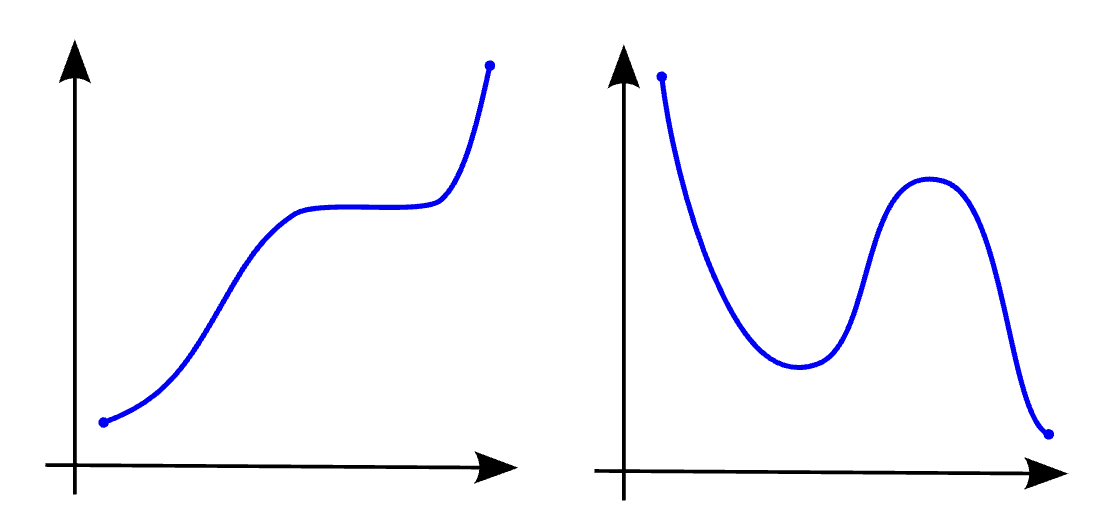
\includegraphics[scale=0.35]{monotone}


\tiny \href{https://commons.wikimedia.org/w/index.php?curid=2267780}{By Oleg Alexandrov}\end{frame}


\begin{frame}{Changing Variable $Y = f(X)$: 1D}

Assume that $Y$ is a \blu{monotonically increasing} function of $X$. \blu{This just means that $Y$ increase if $X$ increases, and doesn't have turning points.}\\[1ex]
%
$Y=g(X)$\\[1ex]
$X = g^{-1}(Y)$ is the inverse relationship.\\[2ex]
%The inverse function for the Measurements is therefore: $f^{-1}(y) = x$ \\[1ex]
%
We can therefore write:\\[1ex]
$P(Y\leq y) = P( g(X) \leq y ) = P( X \leq g^{-1}(y) ) = P( X \leq x ) $ \\[1ex]

Where $y = g(x) $, so $g^{-1}(y) =g^{-1}(g( x)) = x$.\\[1ex]

\boo{$P(Y\leq y) = P(X\leq x)$}
\end{frame}

\begin{frame}{Changing Variable $Y = f(X)$: 1D}

We have shown that: \boo{$P(Y\leq y) = P(X\leq x)$} \\[1ex]

Therefore the \boo{CDF for $Y$} is:\\[1ex]
$F_Y(y) =  F_X(x)$ \\[1ex]

Therefore the \boo{PDF for $Y$} is:\\[1ex]
$f_Y(y) = \dfrac{d}{dy} F_Y(y) =  \dfrac{d}{dy} F_X( x)=  \dfrac{dx}{dy}  \dfrac{d}{dx} F_X( x) =  \dfrac{dx}{dy}  f_X(x)$ \\[1ex]

%Where we used the chain rule: $\dfrac{dF}{dy} = \dfrac{dF}{dx} \dfrac{dx}{dy} $\\[1ex]

%$f_Y(y) =  \dfrac{dx}{dy}  \dfrac{d}{dx} F_X( x) =  \dfrac{dx}{dy}  f_X(x)$ \\[1ex]

\boo{$f_Y(y) = \dfrac{dx}{dy}  f_X(x)$} \\[1ex]
\end{frame}

\begin{frame}{Changing Variable $Y = f(X)$: 1D}

\boo{$f_Y(y) = \dfrac{dx}{dy}  f_X(x)$} : for a monotonically increasing function \\[1ex]

Generally (monotonic increasing or decreasing):\\[1ex]

$f_Y(y) = \left|\dfrac{dx}{dy} \right| f_X(x)$\\[1ex]

\blu{If the function is not monotonic, we must `divide and conquer': split the function up into ranges over which it is monotonic, and do the transform piece-by piece. See eg \href{https://www.mariushobbhahn.com/2021-05-20-Change_of_variable/}{this blog} for an example.} You don't need this for this module.

%for more see 
\end{frame}


\begin{frame}{Multivariate Transform}

The PDFs $f_X(x)$ and $g_Y(y)$ are multivariate, with $X= \{ X_{(1)}, X_{(2)}   \}$ and similarly for $Y= \{ Y_{(1)}, Y_{(2)} \}$.\\[1ex]

The $X_{(j)}$ are again related to the $Y_{(j)}$, but we now have $Z^2 = 4 $ relationships. Matrices are our friend here.\\

\begin{align*}
\begin{bmatrix}
f_{ Y_{(1)} } \\[1ex]
f_{ Y_{(2)} } \\
\end{bmatrix}
=
\begin{vmatrix}
%\dfrac{\partial \rvX{1} }{\partial \rvY{1}} & \dfrac{\partial x}{\partial y} \\
\dfrac{\partial \rvx{1}}{\partial \rvy{1}} & \dfrac{\partial \rvx{1} }{\partial \rvy{2}} \\[1ex]
\dfrac{\partial \rvx{2} }{\partial \rvy{1}} & \dfrac{\partial \rvx{2} }{\partial \rvy{2}} \\[1ex]
\end{vmatrix}
\begin{bmatrix}
f_{ X_{(1)} } \\[1ex]
f_{ X_{(2)} } \\
\end{bmatrix}
\end{align*}


Equivalently, we can write $f_Y = \dfrac{1}{J} f_X$ where J is the \boo{Jacobian of $Y$}.
\end{frame}
%=

\begin{frame}{The Jacobian}

The \boo{Jacobian of $Y$} is the \textbf{Determinant} of the $Z^2$ matrix of partial derivatives $\dfrac{\partial \rvy{j}}{\partial \rvx{j}}$. 

This allows us to make transforms between variables in multivariate PDFs.\\[1ex]

$f_Y = \dfrac{1}{J} f_X$\\[2ex]


$J = \begin{vmatrix}
\dfrac{\partial \rvy{1}}{\partial \rvx{1}} &  \dots & \dfrac{\partial \rvy{1} }{\partial \rvx{Z}}\\[1ex]
\vdots & \ddots & \vdots \\[1ex]
\dfrac{\partial \rvy{Z} }{\partial \rvx{1}} &  \dots & \dfrac{\partial \rvy{Z} }{\partial \rvx{Z}} \\[1ex]
\end{vmatrix}
$


\end{frame}

\begin{frame}{Jacobian: Example}
\small

Suppose points are randomly distributed in a Cartesian $(x,y)$ plane. How are they distributed in polar coordinates $(r,\theta)$?\\[1ex]

\boo{Relationships}:\\[1ex]
$r = (x^2 +y^2)^{1/2}$\;,\;\; $\theta = \arctan{\dfrac{y}{x}}$\\[1ex]

\boo{Partial Derivatives}:\\[1ex]
\begin{columns}
\begin{column}{0.5\textwidth}
$\dfrac{\partial r}{\partial x} = \dfrac{1}{2}(x^2+y^2)^{-\frac{1}{2}}\cdot 2x$\\[1ex]
$\dfrac{\partial r}{\partial y} = \dfrac{1}{2}(x^2+y^2)^{-\frac{1}{2}}\cdot 2y$\\[1ex]
\end{column}
\begin{column}{0.5\textwidth}
$\dfrac{\partial \theta}{\partial x} = \dfrac{1}{1+(\frac{y}{x})^2}\cdot\left (-\dfrac{y}{x}\right)$\\[1ex]
$\dfrac{\partial \theta}{\partial y} = \dfrac{1}{1+(\frac{y}{x})^2}\cdot\dfrac{1}{x}$\\[1ex]
\end{column}
\end{columns}
\end{frame}

\begin{frame}{Jacobian: Example cont.}
\small
\begin{multicols}{2}
\boo{Jacobian}:\\[1ex]
$J= \begin{vmatrix}
\frac{\partial r}{\partial x} & \frac{\partial r}{\partial y}\\
\frac{\partial \theta}{\partial x} & \frac{\partial \theta}{\partial y}\\
\end{vmatrix} = \frac{\partial r}{\partial x} \cdot \frac{\partial \theta}{\partial y} - \frac{\partial r}{\partial y}\cdot \frac{\partial \theta}{\partial x} = \dfrac{1}{r}$\\[2ex]


\boo{Think}:\\[1ex]
$f(r,\theta) = r\cdot g(x,y)$: this tells us that if $g(x,y)$ is uniform, then $f(r,\theta)$  is linearly increasing with $r$.\\
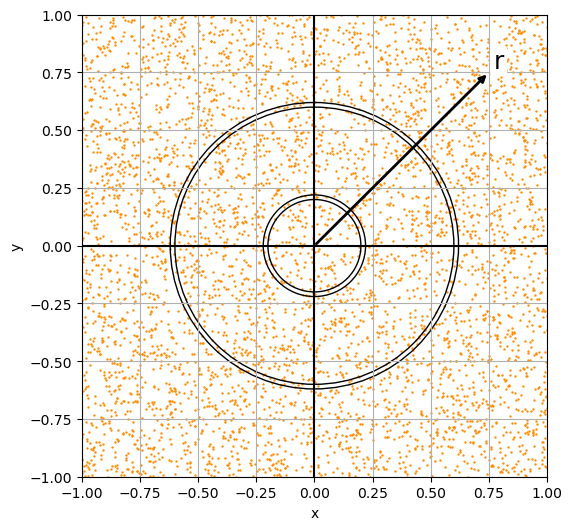
\includegraphics[scale=0.3]{PLOTDAT4-CartesianToPolar.png}
\end{multicols}
\end{frame}





%$\dfrac{dy_{(j)}}{dz_{(j)} }$ provides the relationship allowing us to \boo{Transform} from one RV to the other.\\[1ex]
%
%$f_X(x)  = \dfrac{1}{\mathsf{det}(J)} g_Y(y) $\\[1ex]
%
%The equality assumes that the transformation is single-valued and the interval $y,y+dy$ transforms to $z,z+dz$\\[1ex]






\begin{frame}{Thanks For Your Time}
\center
\Huge
Fin.
\end{frame}






\end{document}